%coding:utf-8

%----------------------------------------
%FOSAPHY, a LaTeX-Code for a summary of linear systems and regulation
%Copyright (C) 2014, Mario Felder, Michael Fallegger

%This program is free software; you can redistribute it and/or
%modify it under the terms of the GNU General Public License
%as published by the Free Software Foundation; either version 2
%of the License, or (at your option) any later version.

%This program is distributed in the hope that it will be useful,
%but WITHOUT ANY WARRANTY; without even the implied warranty of
%MERCHANTABILITY or FITNESS FOR A PARTICULAR PURPOSE.  See the
%GNU General Public License for more details.
%----------------------------------------

\chapter{Einleitung}

\section{Regelkreis}
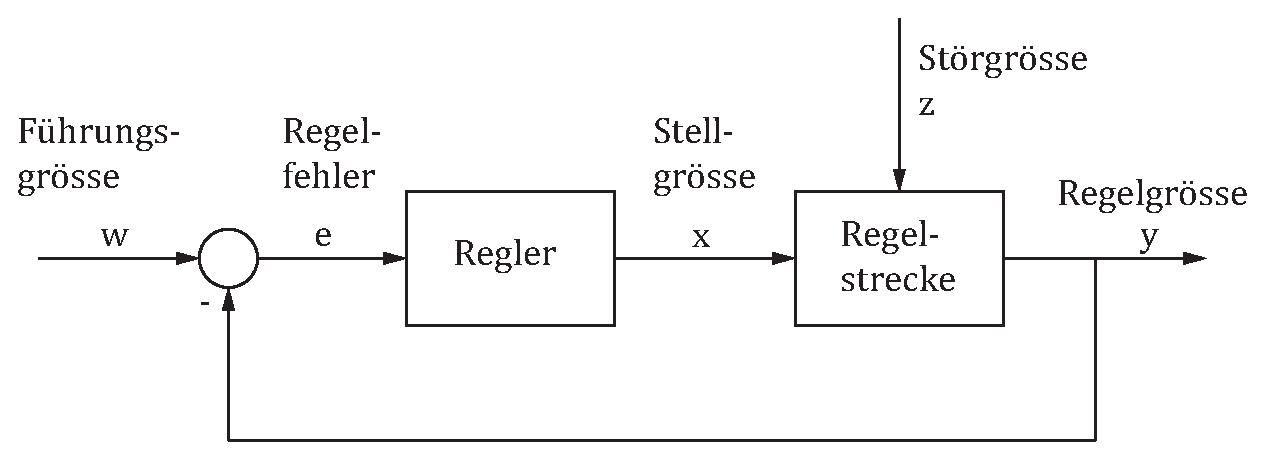
\includegraphics[width = \linewidth]{images/regelkreis.eps}
\\\\
Merkmale:
\begin{itemize}
	\item Erfassen der Regelgrösse $y$
	\item Vergleich von Führungs- und Regelgrösse
	\item Angleichen der Regelgrösse an die Führungsgrösse in Wirkungskreis
\end{itemize}


\section{Systeme}
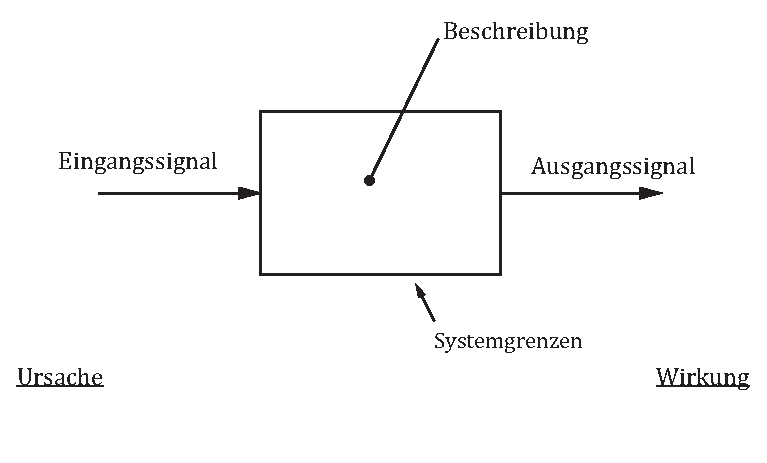
\includegraphics[width = \linewidth]{images/systeme.eps}
\\\\
Signale sind rückwirkungsfrei, also eingeprägte Grössen.
\\\\
\begin{center}
	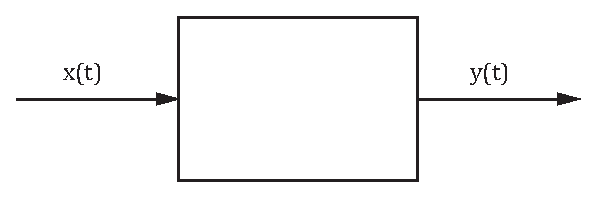
\includegraphics[scale = 0.5]{images/system_bsp.eps}
\end{center}
\begin{tabular}{c|l|l}
 Nr. & Bsp & Klassifikation \\ 
\hline 1 & $y(t) = \cos t \cdot x(t)$ & statisch \\ 
	   2 & $\difrac{y(t)}{t} = - \cos (y(t)) + x(t)$ & \textbf{dynamisch} \\ 
\hline 3 & $\difrac{y(t)}{t} = -y(t) + x(t)$ & \textbf{zeitkontinierlich} \\ 
	   4 & $y((k+1)\tau)=-y(k\cdot \tau) + x(k \cdot \tau)$ & zeitdiskret \\ 
\hline 5 & $y(t) = \cos (x (t-\tau))$ & \textbf{kausal} \\ 
 	   6 & $y(t) = \cos(x(t+\tau))$ & nicht kausal \\ 
\hline 7 & $\difrac{y(t)}{t} = -3y(t) + x(t)$ & \textbf{zeitinvariant} \\ 
	   8 & $\difrac{y(t)}{t} = -\cos t \cdot y(t) +x(t)$ & zeitvariant \\ 
\hline 9 & $\difrac{y(t)}{t} = -y(t) +x(t)$ & \textbf{linear} \\ 
	   10 & $\difrac{y(t)}{t} = -y^2(t) +x(t)$ & nicht linear \\ 
\hline 11 & $\difrac{y(t)}{t} = -y(t) +x(t)$ & \textbf{endlich-dimensional} \\ 
	   12 & $\pdifrac{y(t)}{t} = - \pdifrac{}{x}y(x,t)+x(t)$ & unendlich-dimensional \\ 
\hline 13 & $y(t) = t \cdot \cos^2 t \cdot x(t)$ & \textbf{single input / single output} \\ 
	   14 & $\left[ \begin{matrix} y_1(t) \\ y_2(t) \end{matrix}\right] = \left[ \begin{matrix} -3 & \sin(t) \\ t & -1\end{matrix}\right] \cdot \left[ \begin{matrix} x_1(t)\\ x_2(t) \end{matrix}\right]$ & multiple input / multiple output \\ 
\end{tabular} 
\\\\

\section{Linearisierung}
Approximation durch Gerade:
\[
	f(\bar{x}+\Delta x) \approx \left.(\bar{x})+\difrac{f}{x}\right|_{\bar{x}}\cdot \Delta x
\]

\subsection{Arbeitspunkt festlegen}

Im stationären Zustand gilt:
\[
	\difrac{^n}{t^n} = 0
\]

Für das Eingangssignal $u(t)$ und das Ausgangssignal $y(t)$:
\[
	h(t) = \bar{y} + \Delta y(t) \qquad ,\ u(t) = \bar{u} + \Delta u(t)
\]


\subsection{Linearisierung um Arbeitspunkt}
Es gilt:
\[
	D(y^{(n)}, y^{(n-1)}, \dots ,\dot{y} ,y, u^{(m)}, u^{(m-1)}, \dots , \dot{u} ,u)= 0
\]
$D$ kann am Punkt $\bar{y}, \bar{u}$ approximiert werden durch:
\begin{small}
\[
	\left.\pdifrac{D}{y^{(n)}}\right|_{\begin{scriptsize}\begin{matrix} \bar{y} \\ \bar{u} \end{matrix}\end{scriptsize}} \cdot \Delta y^{n} + \dots +
	\left.\pdifrac{D}{\dot{y}}\right|_{\begin{scriptsize}\begin{matrix} \bar{y} \\ \bar{u} \end{matrix}\end{scriptsize}} \cdot \Delta \dot{y} +
	\left.\pdifrac{D}{y}\right|_{\begin{scriptsize}\begin{matrix} \bar{y} \\ \bar{u} \end{matrix}\end{scriptsize}} \cdot \Delta y +
	\left.\pdifrac{D}{u^{(n)}}\right|_{\begin{scriptsize}\begin{matrix} \bar{y} \\ \bar{u} \end{matrix}\end{scriptsize}} \cdot \Delta u^{n} + \dots +
	\left.\pdifrac{D}{u}\right|_{\begin{scriptsize}\begin{matrix} \bar{y} \\ \bar{u} \end{matrix}\end{scriptsize}} \cdot \Delta u = 0
\]
\end{small}

\begin{center}
	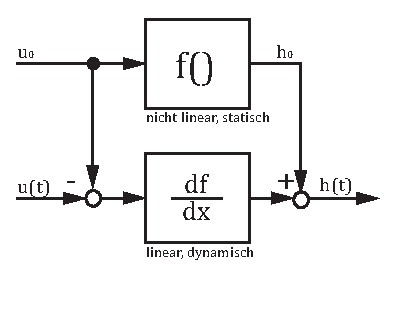
\includegraphics[scale = 0.8]{images/linearisierung.eps}
\end{center}
